\documentclass[spanish, fleqn]{article}
\usepackage{babel}
\usepackage[utf8]{inputenc}
\usepackage{amsmath}
\usepackage{amsfonts}
\usepackage{wasysym}
\usepackage[colorlinks, urlcolor=blue]{hyperref}
\usepackage[top = 2.5cm, bottom = 2cm, left = 2cm, right = 2cm]{geometry}
\usepackage{listings}
\usepackage{color}
\usepackage{graphicx}
%\usepackage{tikz}
%\usetikzlibrary{plotmarks}
\definecolor{gris}{rgb}{0.2,0.2,0.2}

\renewcommand{\thefootnote}{\fnsymbol{footnote}} %Robado de TALF

\title{ILI 285 \\ Laboratorio \#4}
\author{Alonso Sandoval Acevedo\\asandova@alumnos.inf.utfsm.cl\\201073011-5 \and 
		Hernán Vargas Leighton\\hvargas@alumnos.inf.utfsm.cl\\201073009-3}
\date{\today}

\begin{document}
\maketitle

\thispagestyle{empty}

\section{Descripción del experimento}
	%Descripción del experimento y suposiciones
	En primer lugar se ampliará una imagen utilizando las funciones
	interpoladoras, esperamos que el resultado sea optimo para los splines,
	pero creemos que con Newton obtendremos ruido debido al	fenómeno de Runge.\\
	En la segunda parte analizaremos los beneficios y contras al utilizar puntos
	de Chebyshev para aproximar una función. Observaremos que es lo que ocurre
	al aumentar los puntos óptimos utilizados, como también veremos como afecta
	la variación del	parámetro $\alpha$  de la función al error de  la
	interpolación.

\section{Desarrollo}
	%Desarrollo y análisis de resultados
	\subsection{Image Resizing}
	\begin{enumerate}
		\item[a)]
			La estrategia utilizada para agrandar las imágenes consiste en
			aplicar una función de interpolación para filas y luego columnas,
			en este caso se utilizó la función \texttt{interpol1d} de
			\texttt{scipy.interpolate} para splines cúbicos y, para las 
			diferencias divididas de Newton, se modifico en menor medida el
			código de Ernesto P. Adorio, obtenido en la página web 
			\texttt{http://adorio-research.org}. \\
			El algoritmo toma los pixeles de la imagen original y los
			distribuye equis-espaciados en la nueva imagen. En los puntos en
			los cuales no se tiene información, se utiliza la función elegida
			para interpolar su valor. Este proceso se hace primero para todas
			las lineas y, una vez terminado, tendremos una imagen expandida solo
			en una de sus dimensiones, es decir $A^{m\times n} \rightarrow
			A^{m\times n\cdot L}$ siendo $L$ la razón de expansión. En este
			caso, con splines cúbicos y expandiendo a 5X tenemos:
			\begin{figure}[ht!]
				\centering
				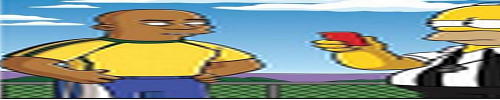
\includegraphics[width=200px]{Graficos/5xhomero_spline_media.png}
				\caption{Expansión de una dimensión}
			\end{figure}
			\\Para una imagen $A^{m\times n}$ este proceso conlleva el calculo
			de $m$ funciones interpoladoras, además debemos evaluar dichas
			funciones por cada uno de los pixeles de la nueva imagen, es decir,
			$n\cdot L$ veces cada función, $n\cdot L\cdot m$ evaluaciones en
			total.\\
			Tomando ésta como la nueva imagen a expandir, nos basta repetir el
			proceso pero ahora para las columnas y  con ello conseguiremos la 
			imagen expandida final.\\
			En el proceso de expansión de de $A^{m\times n\cdot L} \rightarrow 
			A^{L(m\times n)}$ tenemos que calcular $n\cdot L$
			funciones interpoladoras y evaluar cada una de ella en $m\cdot L$
			puntos, en total $m\cdot n\cdot L^{2}$ evaluaciones.\\
			\newpage
			Las imágenes resultantes serán:
			\begin{figure}[ht!]
				\begin{minipage}[b]{0.5\linewidth}
					\centering
					
\includegraphics[width=200px]{Graficos/5xhomero_spline.png}
					\caption{Splines cúbicos}
				\end{minipage}
				\begin{minipage}[b]{0.5\linewidth}
					\centering
					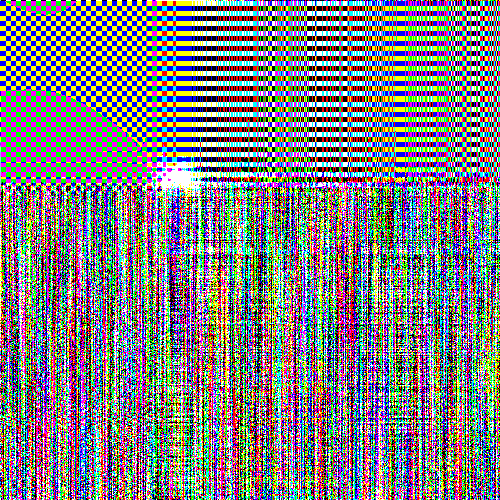
\includegraphics[width=200px]{Graficos/5xhomero_newton.png}
					\caption{Diferencias divididas de Newton}
				\end{minipage}
			\end{figure}
			\\Como podemos ver que el proceso con splines cúbicos da los
			resultados esperados, pero para Newton solo obtenemos ruido.
			Creemos que este problema sucede debido al fenómeno de Runge,
			mientras más puntos tenemos, el error de la interpolación entre
			ellos aumentará considerablemente.\\
			Nuestro algoritmo esta escrito de manera que si encuentra un valor
			mayor a $255$ o menor a $0$ simplemente escriba en la matriz un 
			$255$ o $0$ respectivamente, así se podrá siempre generar una
			imagen, es por ello que, a pesar de que los valores de interpolación
			de Newton deberían salir del rango de representación \texttt{RGB},
			podemos ver este ruido.\\
			El gran problema que encontramos a la hora de agrandar las imágenes
			fue el tiempo que demora el algoritmo en hacer la ampliación. Para
			analizar este factor primero debemos recordar que el proceso
			completo necesitará:
			\begin{itemize}
				\item
					$m + n\cdot L$ funciones interpoladoras.
				\item
					$n\cdot m\cdot(L+L^{2})$ evaluaciones de dichas funciones.
			\end{itemize}
			Sin considerar el tiempo que se gasta en las asignaciones de memoria
			y cálculos menores.\\
			Para la imagen suministrada tenemos que la resolución es de
			$100\times 100$ pixeles y queremos una ampliación \texttt{5X}, es
			decir $m=100$, $n=100$ y $L=5$, reemplazando en las formulas
			tenemos que necesitaremos calcular $600$ funciones interpoladoras y
			evaluar $350000$ veces en total. Para la interpolación con splines
			cúbicos tenemos que, en el computador que trabajamos\footnotemark[1],
			para obtener una función de interpolación se demora aproximadamente
			$0.013$ segundos, mientras que para evaluarla demoró cerca de 
			$0.00015$ segundos. Con estos tiempos tenemos que las obtención de
			las funciones interpoladoras demorará cerca de $8$ segundos y la 
			evaluación de estas tomará $53$ segundos aproximadamente, con ello
			concluimos que el algoritmo demorará al menos $61$ segundos, y ello
			sin tener en cuenta el resto de los cálculos y el trabajo de
			memoria.\\
			\footnotetext[1]{Dell-xps-15: Intel Core i7 CPU Q 740 @ 1.734GHz, 
			6GB 1333Mhz DDR3}
			Creemos que esta es una de las principales razones por las cuales el
			algoritmo es lento. Para solucionar este problema podríamos pensar
			en algún algoritmo que interpole ambas dimensiones al mismo tiempo,
			o mejor aún, aprovechando que el calculo de las funciones
			interpoladoras y su aplicación en la respectiva fila/columna es
			independiente de las demás, podríamos hacer el proceso utilizando
			multi-procesamiento, de esta manera obtener y evaluar paralelamente
			todas las funciones interpoladoras de las filas y luego hacer lo 
			mismo para las columnas.
	\end{enumerate}

\newpage 
	\subsection{Puntos de Chebyshev}
	\begin{enumerate}
		\item[a)]
			Gráficos de $f(x,1)$ y $P_n(x)$\\
			\begin{figure}[ht!]
				\centering
				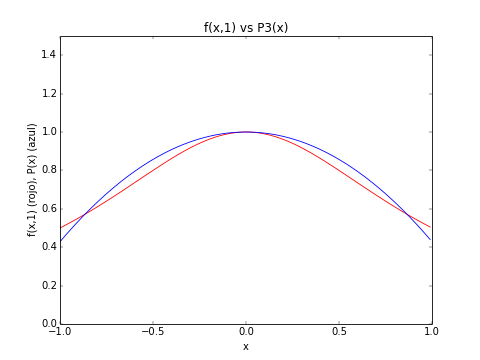
\includegraphics[width=162px]{Graficos/pol3.png}
				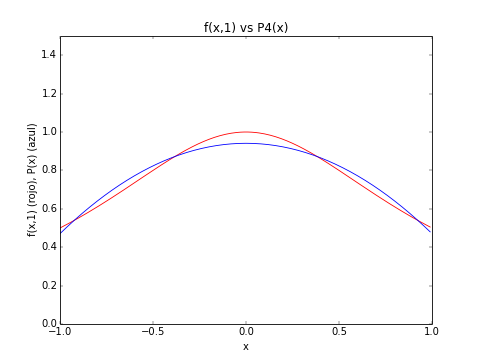
\includegraphics[width=162px]{Graficos/pol4.png}
				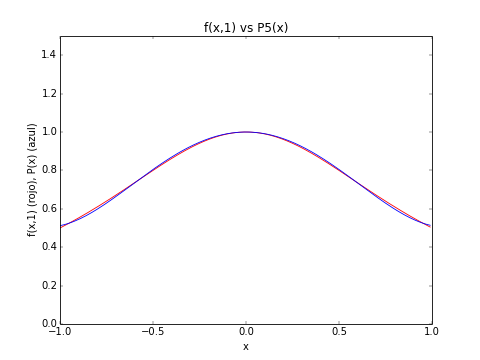
\includegraphics[width=162px]{Graficos/pol5.png}
			\end{figure}
			\begin{figure}[ht!]
				\centering
				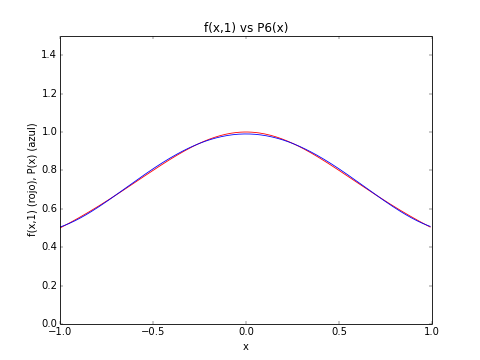
\includegraphics[width=162px]{Graficos/pol6.png}
				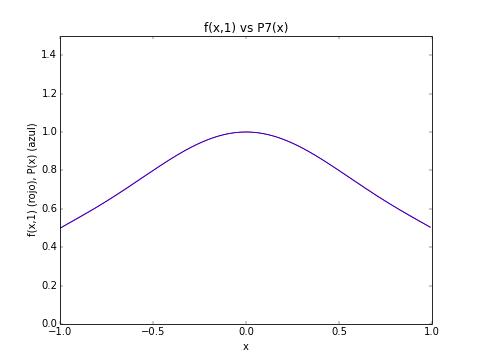
\includegraphics[width=162px]{Graficos/pol7.png}
			\end{figure}
			\\Para la interpolación utilizamos el método
			diferencias divididas de Newton, programado por 
			nosotros, en conjunto a los $n$ puntos de 
			Chebyshev con los cuales evaluamos en $f(x,1)$ y
			generamos los datos que nos permiten interpolar la 
			función. 
			\\Es evidente en los gráficos que al aumentar el 
			número de puntos de Chebyshev mejora la 
			aproximación de la función interpoladora(Azul).
		\item[b)]
			Gráfico del error en escala logarítmica versus el
			número de puntos de Chebyshev, $n = 3:7$.
			\begin{figure}[ht!]
				\centering
				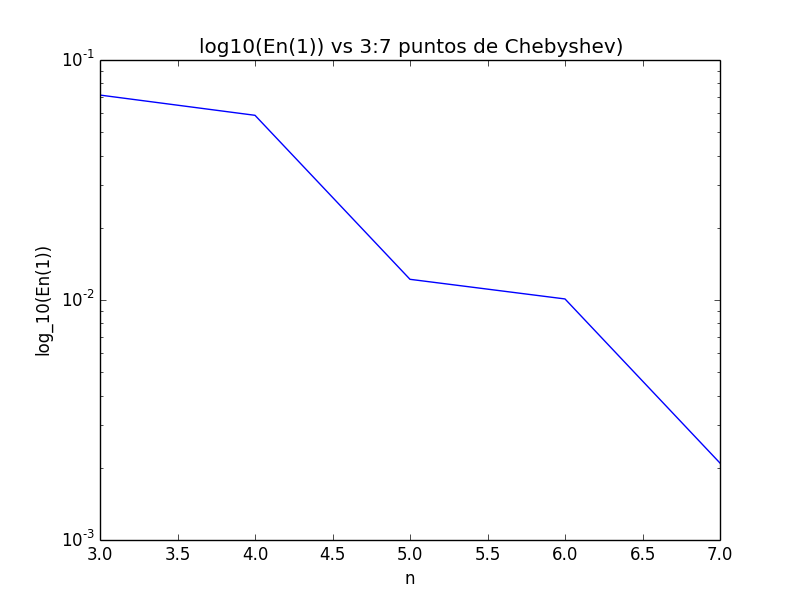
\includegraphics[width=200px]{Graficos/Error-vs-n.png}
			\end{figure}
			\\El gráfico es condescendiente con los resultados del 
			punto anterior, a medida que se aumentan los puntos de 
			Chebyshev, el error entre la función original y su 
			interpolación disminuye, es decir mejora la aproximación
			de $P(x)$ a $f(x,1)$. Notar que la pendiente es negativa
			a simple vista, un cálculo aproximado de la pendiente 
			(mediante regresion lineal en python) nos da un valor 
			de: $s: -2,43$
\newpage
		\item[c)]
			Gráfico de la pendiente del error versus el $\alpha$
			de la función $f(x, \alpha)$
			\begin{figure}[ht!]
				\centering
				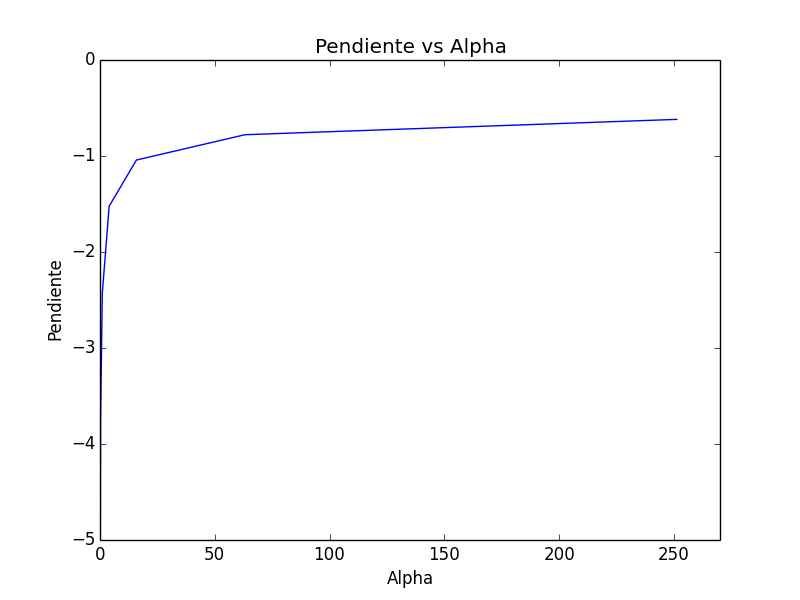
\includegraphics[width=300px]{Graficos/SvsA.png}
			\end{figure}
			\\Según nuestro gráfico es mejor un $\alpha$ pequeño, 
			dado
			que la pendiente del gráfico es más negativa y por lo 
			tanto, el error disminuye más rapido a medida que 
			aumentamos los puntos de Chebyshev (hasta una cierta 
			cantidad). A mayor valor de $\alpha$, menor es la 
			pendiente del error, y por lo tanto, los puntos de 
			Chebyshev se hacen menos significativos (La pendiente
			del error tiende a 0, por tanto el error practicamente
			no varia para $\alpha$ grande).

		\item[d)]
			Gráfico del error en escala logarítmica versus el número
			de puntos de Chebyshev, $n = 2:50$.
			\begin{figure}[ht!]
				\centering
				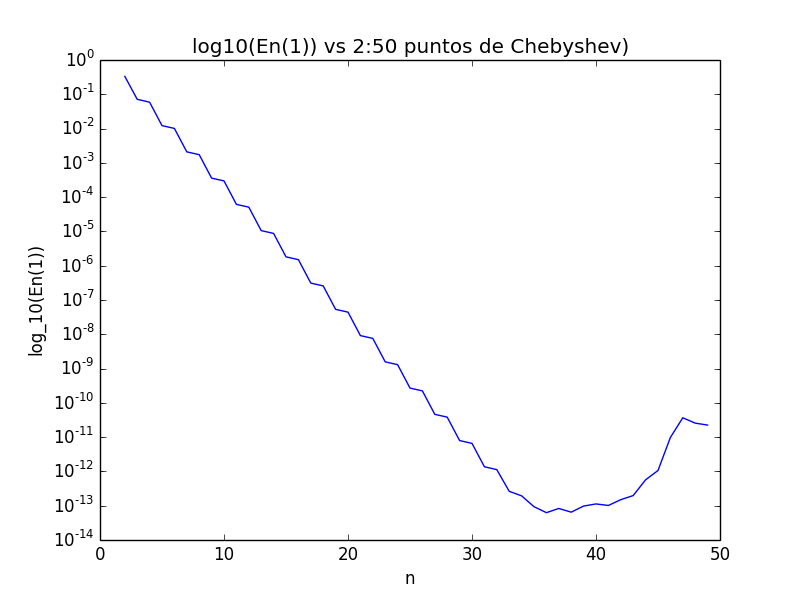
\includegraphics[width=300px]{Graficos/Error-vs-n2.png}
			\end{figure}
			\\El gráfico del error se comporta normalmente hasta
			valores cercanos a $10^{-14}$, aproximadamente 40 puntos
			de Chebyshev, posteriormente los valores del error 
			comienzan a aumentar  nuevamente, ¿por qué?, pensamos que
			se debe a la representación computacional, por ejemplo,
			para valores muy pequeños de Chebyshev, pueden ocurrir
			errores de cancelación o cifras significativas en el 
			algoritmo diferencias divididas de Newton, lo cual 
			arruina la interpolación.
	\end{enumerate}
\newpage
\section{Conclusiones}
	Con respecto al proceso de agrandar imágenes podemos concluir que si bien
	nuestro algoritmo logra el resultado esperado en el caso de splines cúbicos
	se demora demasiado, por lo cual, no debe ser la manera en la cual se hace
	este proceso actualmente. Por otro lado, vemos que Newton no es un buen
	método de interpolación para las imágenes debido al fenómeno de Runge.\\
	Para la sección dos concluimos que a mayor cantidad de puntos de Chebyshev
	mejor es la interpolación, sin embargo, sobre cierta cantidad, 40 en nuestro
	caso, el error deja de disminuir y comenzará a crecer, creemos que uno de 
	los causantes de este fenómeno son valores computacionales muy pequeños en
	los puntos de Chebyshev los que hacen divergir a la función, afectando al
	algoritmo de D.D de Newton.\\
	Otro enfoque es el fenómeno de Runge, el cual podemos ver en el siguiente
	gráfico:
	\begin{figure}[ht!]
		\centering
		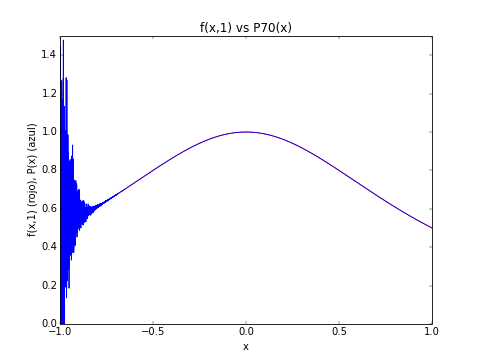
\includegraphics[width=250px]{Graficos/Runge.png}
	\end{figure}
	\\Por ultimo, la interpolación también dependerá de la función, en nuestro
	caso, a mayor $\alpha$ para $f(x,\alpha)$ menor es el impacto de los puntos
	de Chebyshev, por lo que la pendiente del error decrece.
\section{Fuentes}
	\begin{itemize}
		\item
			\textbf{scipy - interp1d:} Sobre la función utilizada para
			interpolar con splines cúbicos, enlace: 
			\url{http://docs.scipy.org/doc/scipy/reference/generated/scipy.interpolate.interp1d.html}
		\item
			\textbf{Adorio-research.org - Newton interpolating polynomial for
			approximations:} Fuente de la función utilizada para interpolar
			con diferencias divididas de Newton en la primera parte, enlace:
			\url{http://adorio-research.org/wordpress/?p=11165}
	\end{itemize}

\newpage
\section{Anexo}
	%hack para acentos:
	\lstset{literate=
		{á}{{\'a}}1 {é}{{\'e}}1 {í}{{\'i}}1 {ó}{{\'o}}1 {ú}{{\'u}}1
		{Á}{{\'A}}1 {É}{{\'E}}1 {Í}{{\'I}}1 {Ó}{{\'O}}1 {Ú}{{\'U}}1
		{à}{{\`a}}1 {è}{{\'e}}1 {ì}{{\`i}}1 {ò}{{\`o}}1 {ù}{{\`u}}1
		{À}{{\`A}}1 {È}{{\'E}}1 {Ì}{{\`I}}1 {Ò}{{\`O}}1 {Ù}{{\`U}}1
		{ä}{{\"a}}1 {ë}{{\"e}}1 {ï}{{\"i}}1 {ö}{{\"o}}1 {ü}{{\"u}}1
		{Ä}{{\"A}}1 {Ë}{{\"E}}1 {Ï}{{\"I}}1 {Ö}{{\"O}}1 {Ü}{{\"U}}1
		{â}{{\^a}}1 {ê}{{\^e}}1 {î}{{\^i}}1 {ô}{{\^o}}1 {û}{{\^u}}1
		{Â}{{\^A}}1 {Ê}{{\^E}}1 {Î}{{\^I}}1 {Ô}{{\^O}}1 {Û}{{\^U}}1
		{œ}{{\oe}}1 {Œ}{{\OE}}1 {æ}{{\ae}}1 {Æ}{{\AE}}1 {ß}{{\ss}}1
		{ç}{{\c c}}1 {Ç}{{\c C}}1 {ø}{{\o}}1 {å}{{\r a}}1 {Å}{{\r A}}1
		{€}{{\EUR}}1 {£}{{\pounds}}1 {ñ}{{\~n}}1
	}

%Anexo con código utilizado
	\lstinputlisting[language=Python,
				 frame=single,
				 showstringspaces=false,
				 commentstyle=\color{gris},
				 title=\lstname,
			 	 tabsize=4]{../Codigos/Laboratorio4.py}

\vfill\hfill HV/AS/\LaTeXe
\end{document}
